\documentclass{article}
\usepackage{titling}
\usepackage{float}
\usepackage{wrapfig}
\usepackage{graphicx}
\usepackage{hyperref}
\renewcommand{\figurename}{Figur}
\title{Projekt TicTacToe}
\author{Albin Frick}
\def\inst{tillämpad fysik och elektronik}
\def\typeofdoc{Report}
\def\course{Applikationsutveckling för internet vt19}
\def\title{Lab rapport}
\def\namea{Albin Frick}
\def\emaila{\usernamea{}{}@cs.umu.se}
\def\graders{Per Kvarnbrink, Stefan Berglund}
\begin{document}
	\begin{titlepage}
		\thispagestyle{empty}
		\begin{large}
			\begin{tabular}{@{}p{\textwidth}@{}}
				\textbf{UMEÅ UNIVERSITY \hfill \today} \\
				%\textbf{\typeofdoc} \\
			\end{tabular}
		\end{large}
		%\vspace{10mm}
		\begin{center}
			\vspace{15mm}
			\large{\course} \\
			\vspace{5mm}
			\huge{\textbf{Laboration1}}\\
			\vspace{5mm}
			\large{\emph{API med Alternativt Gränssnitt}}\\
			\vspace{10mm}
			\large{\theauthor}
		\end{center}
		\begin{center}
			\vfill
			\large{\textbf{Handledare}}\\
			\vspace{1mm}
			\large{\graders}
		\end{center}

	\end{titlepage}
\newpage
\tableofcontents
\newpage
\section{Inledning}%
\label{sec:inledning}
Denna laboration har gått ut på att bekanta sig med node.js och react.js.
Jag valde att bygga mitt API med hjälp av node.js och det konsumerande gränssnittet med react.js.
Jag valde att använda både node och react för att jag ansåg det var ett effektivt sätt att lära mig två olika ramverk.\\

\noindent
Jag har valt att göra uppgiften på plus-nivå.

\section{Problembeskrivning}%
\label{sec:problembeskrivning}
För att få detta att fungera måste det finnas tre huvudkomponenter.
\begin{itemize}
	\item Databas
	\item Webbserver - API
	\item Webbserver - Konsumerande gränsnitt
\end{itemize}

\noindent
Laborationen gick alltså ut på att skapa dessa tre och få dem att samarbeta på ett tillfredställande sätt.


\section{Systembeskrivning}%
\label{sec:systembeskrivning}
Databasen är byggd i MySQL och består av tre tabeller, Books, Users, BookUserRelation. Bara Books och Users blev använda under laborationen på grund av tids brist. Vid vidare arbetning av API:t skulle de fortfarande gå att använda.\newline
\begin{figure}[H]
	\centering
	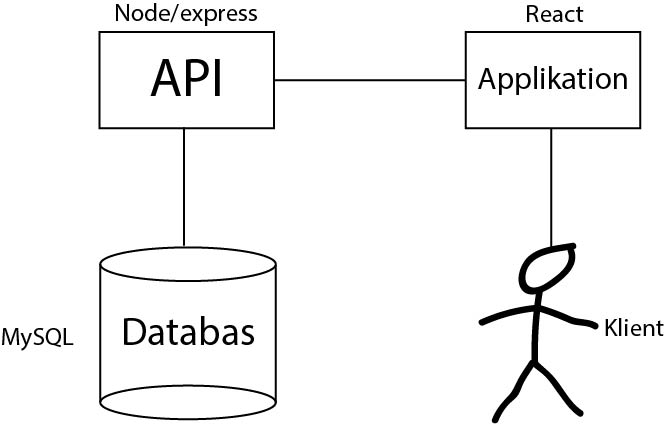
\includegraphics[width=0.8\linewidth]{Images/relation.jpg}
	\caption{Relationen mellan de olika komponenterna}
	\label{fig:}
\end{figure}
\noindent
I figur 1 finns ett ER-schema där man kan se hur databasstrukturen.
\begin{figure}[H]
	\centering
	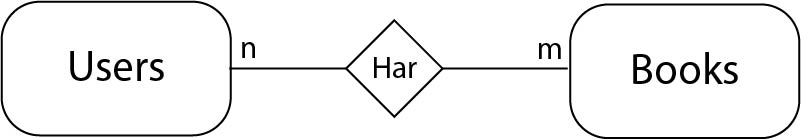
\includegraphics[width=0.8\linewidth]{Images/er-shema.jpg}
	\caption{ER-schema över databasen}
	\label{fig:}
\end{figure}

\noindent
API:t är byggt med hjälp av node.js och express. API:t hämtar, visar och ändrar i databasen. Varje operation sker i en egen "route". Ett exempel på detta går att se i figur 2. 
\begin{figure}[H]
	\centering
	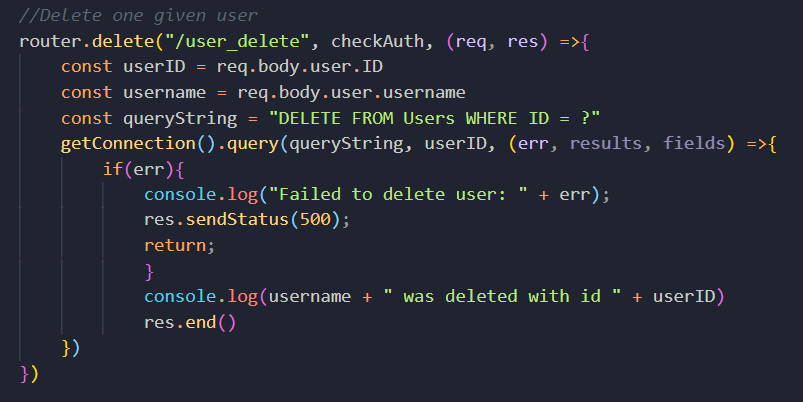
\includegraphics[width=0.8\linewidth]{Images/user_delete_route.PNG}
	\caption{Kod som besrkiver routen /users\_delete}
	\label{fig:}
\end{figure}

\noindent
En "route" är alltså url:en till en viss plats i API:t, som /users, /books mm.
Efter vilket route som är beskriven i figur 2 ser man checkAuth. Denna funktion sköter hanteringen om användaren är inloggad eller inte men mer om det senare.\\
Genom att använda pluginen "mysql" i node så har en koppling gjorts med databasen i funktionen getConnection(). 
När en koppling är gjord kan man då skicka in en förfrågan till databasen. I figur 3 är förfrågan\\

"DELET FROM Users WHERE ID = ?"\newline

\noindent
Frågetecknet agerar som en placeholder för parametern för id:t som skickas med i queryn.
Om det skulle bli något fel vid borttagningen ur databasen kommer en felstatus med 500 att skickas tillbaka som response. 
Blir inget fel kommmer användarnamnet och id att skrivas ut i konsolen.\\

\noindent
Det konsumerade gränssnittet är uppbyggt i react och består av åtta sidor. Alla sidor har samma meny förutom "Login" och "Logout" då detta behövs för att uppdatera inloggningen. 
Från de andra sidorna kan man ta sig till andra sidorna. 
Genom att klicka in på användare t.ex. får man en lista över de användare som finns därifrån kan man välja att radera eller redigera en användare dock fungerar detta enbart om na är inloggad.\\

\noindent
För att skicka eller hämta data mellan API:t och klienten används react pluginen "axios" detta är en förlängning från javascriptets "ajax". Det används för att kunna skicka get-, post-, put- och delete-förfrågningar.\\

\noindent
Dessa förfrågningar är alltså:
\begin{itemize}
	\item get - Hämta information
	\item post - Lägga till information
	\item put - Redigera information
	\item delete - ta bort information
\end{itemize}
\noindent
Genom axios skickas ett objekt av det som ska läggas till, redigeras eller tas bort. Där det krävs inloggning skickas också ett "token" med.\\

\noindent
Validering är gjord på både klient och server. På klientsidan stoppas användaren om den försöker skapa en användare med för kort användarnamn eller glömmer att skriva in ett lösenord t.ex.\\

\noindent
P.g.a. tidsbrist blev det ingen komplett validering på server-nivån. Det finns validering när en användare ska skapas. Då kollas det om användarnamnet redan finns i databasen och ser till så att de inte är null. Denna information skickas också vidare upp till klienten så användaren vet vad den ska göra.\\

\noindent
När något går snett i API:t kommer det att skickas en status kod tillbaka beroende på vad som har hänt.
Det finns väldigt många statuskoder där den mest kända kanske är 404 - not found. Genom en enkel googling kan man få upp listor om vad alla betyder.\\
De statuskoder som har använts mest i denna labb har varit:
\begin{itemize}
	\item 404 - Not Found
	\item 401 - unauthoraized
	\item 500 - Internal Server Error
	\item 200 - OK
\end{itemize}
Första siffran i statusen grupperar den. 
\begin{itemize}
	\item 1 - Informerande 
	\item 2 - Lyckad förfrågan
	\item 3 - Vidarekoppling
	\item 4 - Klientfel
	\item 5 - Serverfel
\end{itemize}
\subsection{Inloggning}%
\label{sub:inloggning}
En inloggning kan vara bra att ha för ett API så inte vem som helst kan komma in och ändra och ta bort grejor. I tidigare kurser har vi använt oss av sessionsvariabler eller något linkande löper ut efter en viss tid. Detta går inte i ett API då den är så kallad "stateless" API:t kan alltså inte veta om någon är inloggad.\\

\noindent
För att lösa detta kan man använda sig av jsonwebtokens, tokens. Dessa token kan genereras till varje användare och kontrolleras API:t.\\

\noindent
När man skapar en ny användare kollar API:t först att det inte finns en användare med samma användarnamn (kanske skulle varit bättre med email, men använde användarnman i mån av tid)
sedan hashas lösenordet med saltning och läggs till i databasen. Allt detta är försståss om ingenting går fel.\\

\noindent
När den nya användaren sedan loggar in kommer användar namnet och lösenordet att jämnföras igen.
'bcrypt' har använts för att hasha och jämföra lösenorden. 
Om allting är OK kommer ett token att signeras.
Det signeras med användarens användarnamn, id och en privat nyckel som är en miljö-varibel (så man inte kan se den i koden). När den signeras sätts också en tid, en timme i detta fall. Till slut returneras responsen med status 200 (OK), ett meddelande att allting gick bra och tokenet.\\

\noindent
För de routes på API:t som enbart användare har åtgång till kontrolleras då detta token varje gång genom en så kallad middelware. Denna kontrollerar det givna token från användaren och den privata nyckeln stämmer allt kommer man vidare till routen annars kommer en status av 401 att skickas tillbaka.\\

\noindent
När användaren loggar in på klientsidan kommer klienten att ta emot det nyssa skapade tokenet och lägga till det i en global variabel. Denna kommer att ligga där till användaren loggar ut. Hinner tokenet löpa ut kommer det att skrivas över då användaren loggar in igen.


\section{Implementation}%
\label{sec:implementation}
Som nämt så har node.js, react.js och MySQL använts för att implementera denna lösning.
Jag ska skrivit både backend och frontend i visual studio code. Genom den integrerade terminalen kunde jag har koll på vad som hände på API och gränssnitts servern. 
För node användes "nodemon". Detta är en plugin som startar om servern varje gång någonting ändras. Detta var till stor hjälp då man gör många ändringar under utvecklingen.\\

\noindent
För att skapa react projectet användes:\\
npx create-react-app\newline
Detta generarar nödvändiga filer och mappar för att komma igång med utvecklingen.\\
\noindent
Byggandet av alla komponenter gick till i följande ordning:
\begin{enumerate}
	\item Databas
	\item API
	\item Konsumerande gränssnitt
\end{enumerate}
API:t testades genom att skapa ett html sida på samma host. 
Sidan kan ses på figur \ref{fig:testsida} och innehåller bara inmatningsfält och knappar.
\begin{figure}[H]
	\centering
	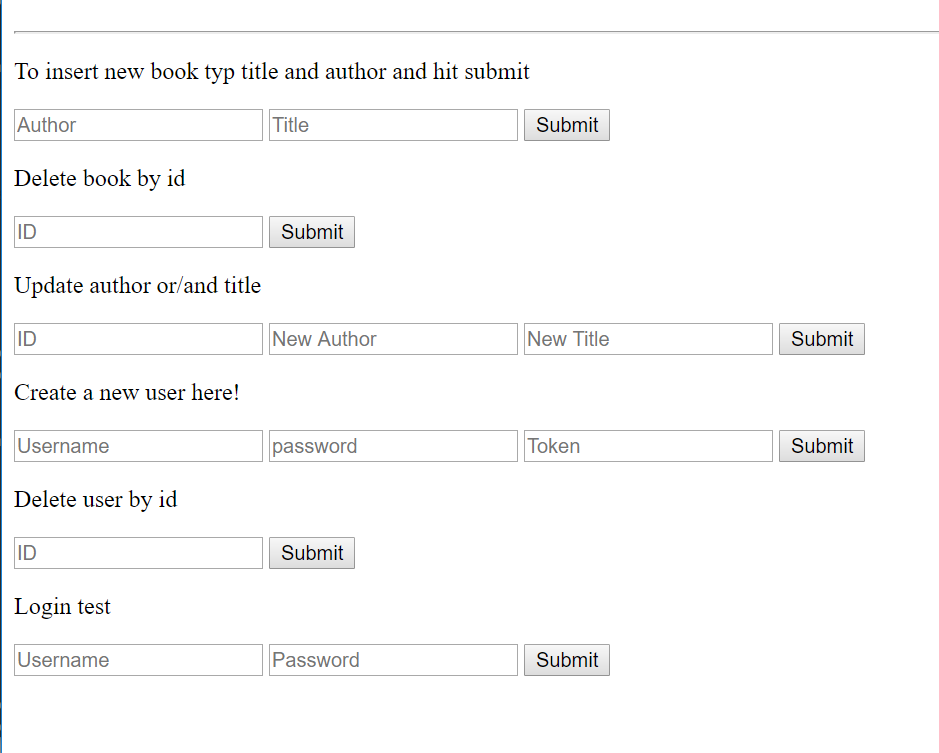
\includegraphics[width=0.8\linewidth]{Images/form.PNG}
	\caption{Testsida för API}
	\label{fig:testsida}
\end{figure}
\noindent
Det hade nog varit bättre att använda sig av något som postman men detta fungerade också.

\section{Gränssnitt}%
\label{sec:gr_nssnitt}
Gränssnittet har varit väldigt simpelt men med en del extra finnesser.
Som man kan se från figur \ref{fig:books} så är det inte väldigt vackert men det kan var användbart. 
\begin{figure}[H]
	\centering
	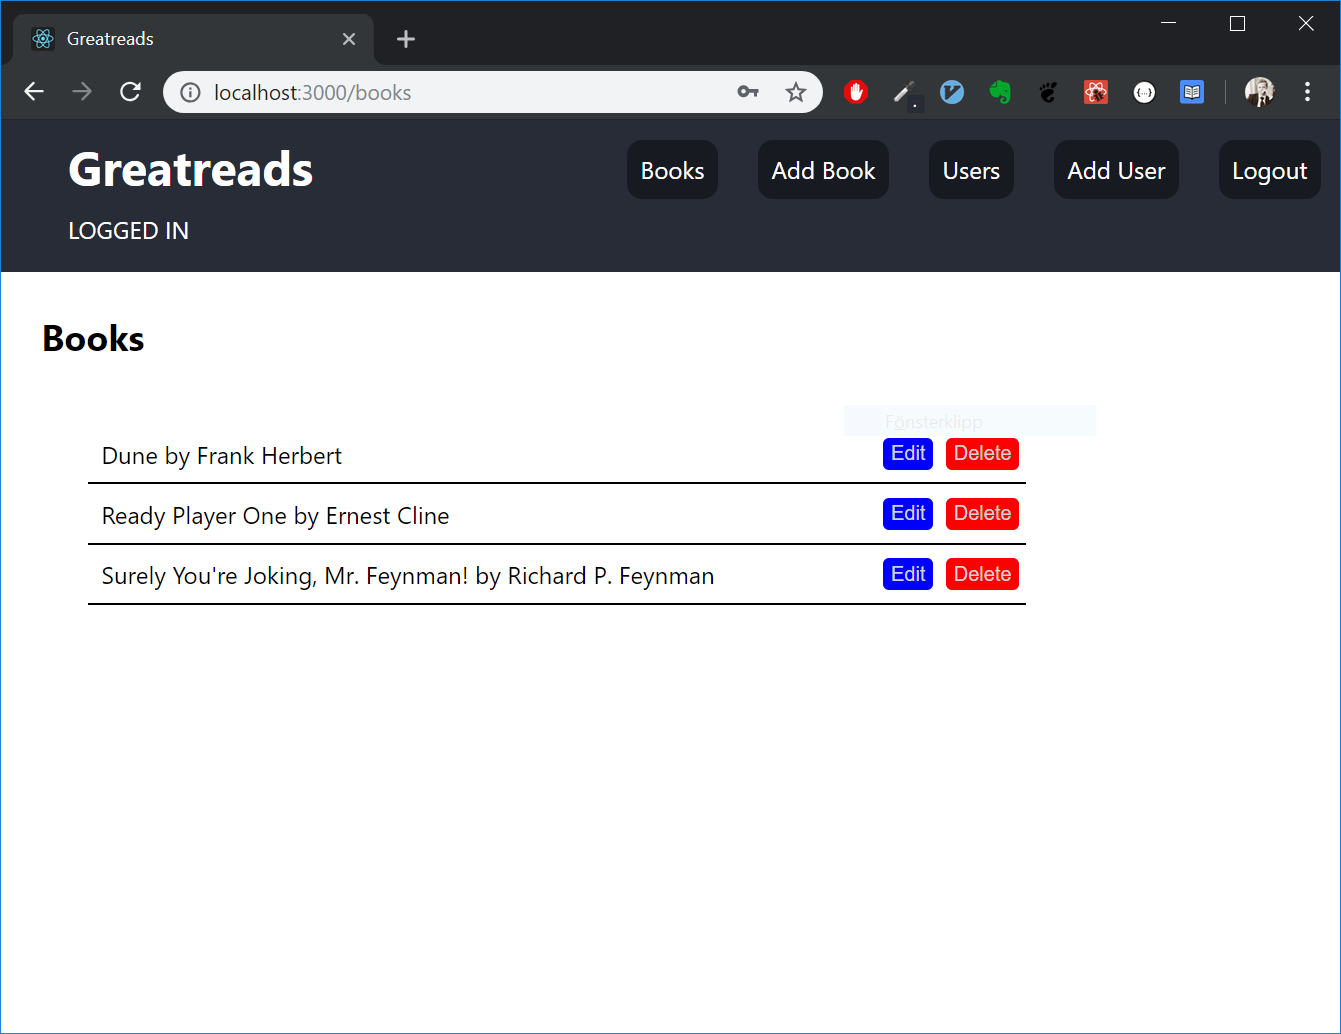
\includegraphics[width=0.8\linewidth]{Images/books.PNG}
	\caption{Lista över böcker}
	\label{fig:books}
\end{figure}
\noindent
Från figur 5 kan man se under loggan att man är inloggad.
Längst till höger finns det också en logga ut knapp. 
Klickar man på den får man logga ut.
Kommer man till listan över användare som figur 6
\begin{figure}[H]
	\centering
	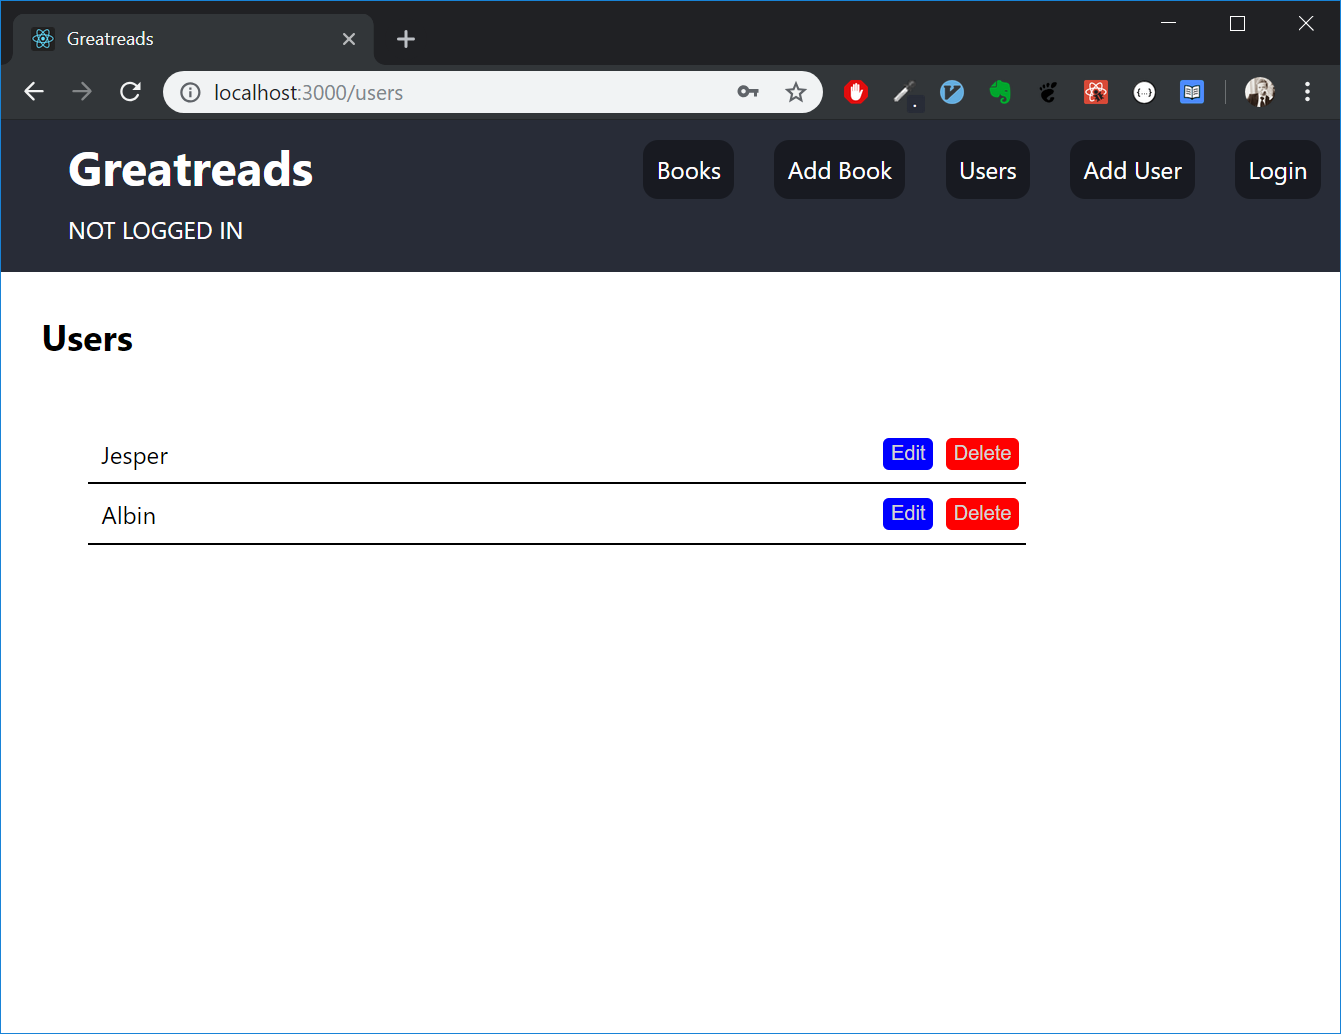
\includegraphics[width=0.8\linewidth]{Images/users.PNG}
	\caption{Lista över användare}
	\label{fig:users}
\end{figure}
\noindent
När man loggat ut kommer knappen för att logga ut att försvinna och ersättas av en logga in knapp. 
Om man försöker att ta bort en bok utan att loggat in kommer det att se ut som på figur 7
\begin{figure}[H]
	\centering
	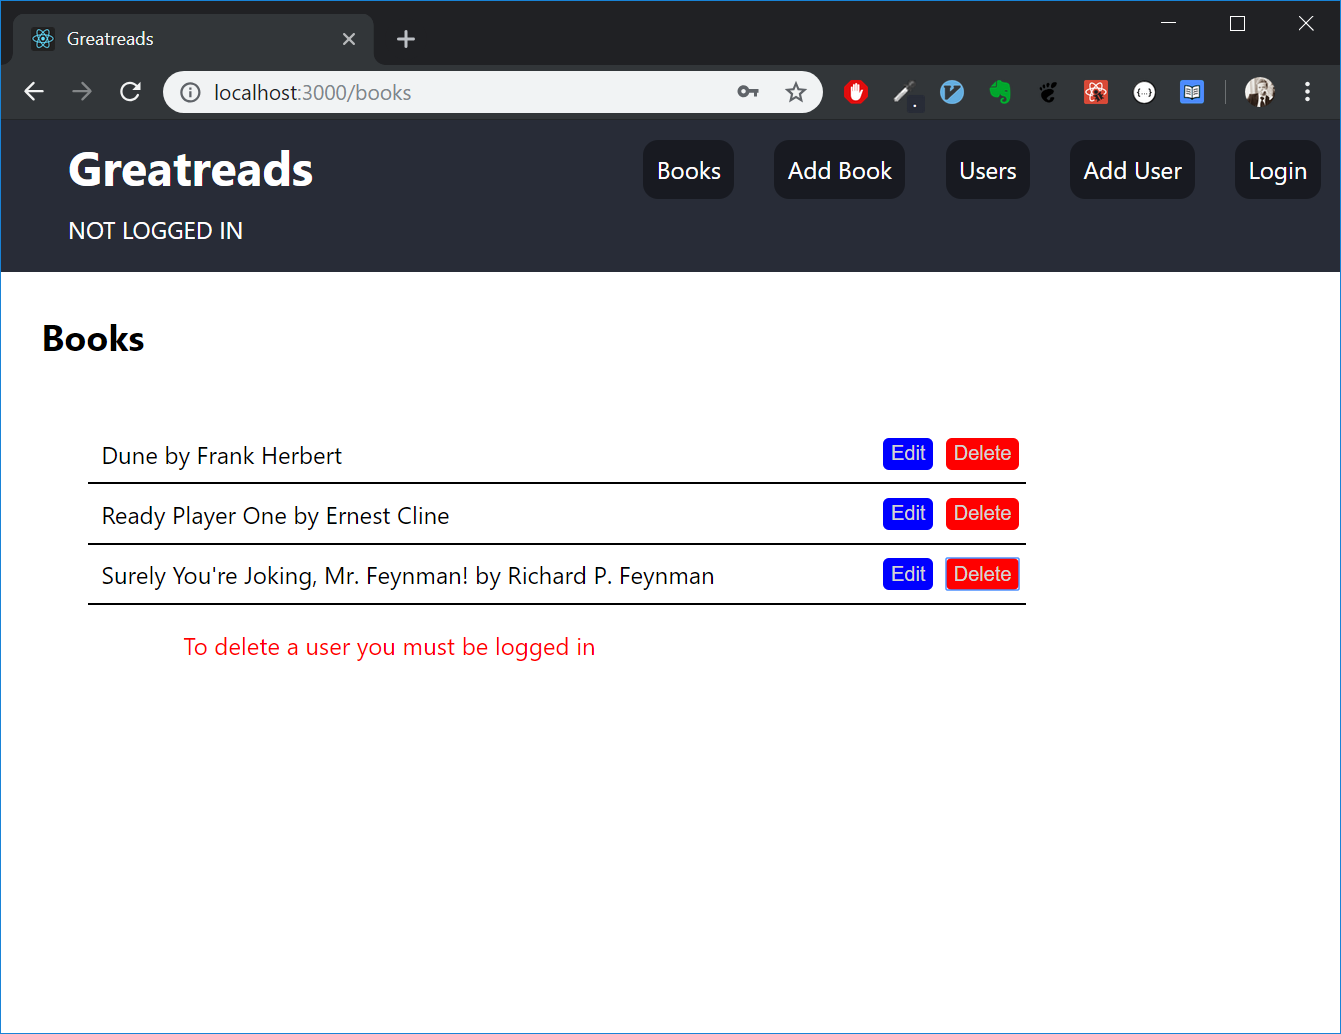
\includegraphics[width=0.8\linewidth]{Images/booksMustLogg.PNG}
	\caption{Felmeddelande då man inte loggat in}
	\label{fig:deletebooks}
\end{figure}
\noindent
Som validering när man skapar en ny användare så måste användarnamnet var fem karaktärer långt och lösenordet åtta. 
\begin{figure}[H]
	\centering
	\includegraphics[width=0.8\linewidth]{Images/addUserFelMedd.PNG}
	\caption{Felmeddelande vid förkorta inputs}
	\label{fig:}
\end{figure}
Försöker man med en användare som redan finns ser det ut som figur 9.
\begin{figure}[H]
	\centering
	\includegraphics[width=0.8\linewidth]{Images/addUserFelMedd2.PNG}
	\caption{Felmeddelande vid samma användarnamn}
	\label{fig:name}
\end{figure}
\noindent
De två sista bilderna är exempel på validering på olika nivåer.
När användaren skriver för kort användarnamn kollas det i klienten.
Detta skulle kunna kollas i API:t men det är ganska onödigt då 
klienten vet hur långt det får vara och kan göra det snabbare och behagligare för användaren.\\

\noindent
Klienten kan inte se in i databasen så därför skickas informationen med det inskrivna användarnamnet och lösenordet till API:t här kontrolleras det och ser att användarnamnet finns. API:t släpper då båda de inskrivna användarnamnet och lösenordet och skickar tillbaka en response med statusen 401 unauthorized och meddelandet: "That username already exist".
Detta är alltså validering på server-nivå för att det inte kan ske på klient-klient nivå.\\

\noindent
Går det att lösa valideringen på klient-nivå är det bättre då det blir mindre jobb för datorn och bättre upplevelse för användaren. 

\section{Lösningens begräsningar}%
\label{sec:l_sningens_begr_sningar}
Lösningen har en del begrännsningar. Just nu kan inte användare välja böcker till sig själva utan bara se alla och lägga till. För att göra detta måste relationstabellen för mellan users och books att implementeras. I mån av tid blev detta inte möjligt.\\

\noindent
Just nu kommer man till en vy där man inte kan se menyn när man loggar in och loggar ut så klickar man på någon av dem finns det ingen återvändo. Detta gjordes för att på ett enklare sätt uppdatera headern med "NOT LOGGED IN" texten och knappen. Detta är också något som är möjligt att fixa genom att skicka information mellan komponenterna i react med hjälp av props. Detta är också något som jag inte fått gjort i mån av tid.\\


\section{Problem och Reflektioner}%
\label{sec:problem_och_reflektioner}
Jag tyckte att denna labb var väldgit rolig och utmanande.
Jag hade sedan tidigare aldrig jobbat i node så det var helt nytt.
React var jag lite bekant med då jag gjort några mindre sidor i det 
men aldrig något som kommunicerar med en databas eller API.\\

\noindent
Jag har lärt mig väldigt mycket om hur JavaScript fungerar, hur http-satser fungerar och speciellt hur man kan skapa en säker inloggning till ett API.
Det var det som tog absolut mest av tiden men gav också mest.\\

\noindent
Jag hade en del problem med att få en koppling mellan databasen och node ibörjan. Det löste sig till slut genom att jag fick byta lösenord till "password" för att det skulle fungera.\\

\noindent
Om jag skulle göra om laborationen skulle jag nog vilja pröva att göra databasen av en mongodb. 
Många av de jag har läst på internet och de videor jag har sätt så har de använt mongodb.
Det verkar vara väldigt smidigt och användbart.

\section{Referenser}%
\label{sec:referenser}
Node och express (ep 1-4) - \url{https://www.youtube.com/watch?v=F7NVpxxmmgM}
React validering - \url{https://www.youtube.com/watch?v=FM2RN8rHCTE}\newline
Node säker inloggning (ep 11-13) -\newline
\url{https://www.youtube.com/watch?v=_EP2qCmLzSE&list=PL55RiY5tL51q4D-B63KBnygU6opNPFk_q&index=11}

\end{document}
